\documentclass{beamer}
\mode<presentation>
{
  \usetheme{Montpellier}
  \usecolortheme{orchid} 
  \usefonttheme{professionalfonts} 
  \setbeamertemplate{navigation symbols}{}
  \setbeamertemplate{caption}[numbered]
} 

\usepackage[english]{babel}
\usepackage[utf8]{inputenc}
\usepackage[T1]{fontenc}
\usepackage{textcomp}
\usepackage{braket}
\usepackage{graphicx}
\usepackage{pgfplots}
\usepackage[style=authortitle,backend=biber]{biblatex}
\addbibresource{PresBib.bib}
\usepackage{booktabs}
\usepackage{adjustbox}
\usepackage[font={small}]{caption}
\usepackage{perpage}
\MakePerPage{footnote}
\MakePerPage{fullfootnote}
\usepackage{nicefrac}
\usepackage{mathtools}
\usepackage{bm}


\title[Accelerated Dynamics in HMC Simulations of Lattice Field
Theory]{Accelerated Dynamics in HMC Simulations of Lattice Field
Theory}
\author{Jack Frankland}
\institute{University of Edinburgh}
\date{\today{}}

\begin{document}

\begin{frame}
    \titlepage
\end{frame}

\section{Introduction}

\begin{frame}{Introduction}
    \begin{itemize}
  \item<1-> What are we  doing? 
    \begin{itemize}
        \item<2-> Calculating properties of Quantum Mechanical Systems.
    \end{itemize}
  \item<3-> How are we doing it?
    \begin{itemize}
        \item<4-> Using MCMC (Markov chain Monte Carlo) methods.
    \end{itemize}
  \item<5-> What results have we got?
  \begin{itemize}
        \item<6-> Successfully reproduced harmonic and enharmonic oscillator properties.
    \end{itemize}
  \item<7-> Why are we doing it?
  \begin{itemize}
    \item<8-> Can be used for calculations in lattice field theory.
  \end{itemize}
    \end{itemize}
\end{frame}

\section{Theory}

\begin{frame}{Theory - The Path Integral}
    \only<2-4>
    {
       \begin{block}{Transition Amplitude}
            \only<2-4>
            {
                \begin{equation}
                    \braket{x_b,t_b|x_a,t_a} = \int^{x_b}_{x_a} {\cal D}{x} \exp{\left(\nicefrac{iS\left[{x\left(t\right)}\right]}{\hbar}\right)}
                \end{equation}
            }
            \only<3-4>
            {
                \begin{equation}
                \int^{x_b}_{x_a} {\cal D}{x} = \lim_{N \to \infty} A_N \prod_{n=1}^{N-1} \int^{\infty}_{- \infty} d x_n
                \end{equation}
            }
        \end{block}
    }
    \only<4>
    {
        \begin{block}{Minkowski Action}
            
            \begin{equation}
                    S = \int^{t_b}_{t_a}dt \left[\frac{1}{2}m\left(\frac{dx}{dt}\right)^2 - V(x)\right]
            \end{equation}
            
        \end{block}
    }
    \only<5>
    {
        \centering
        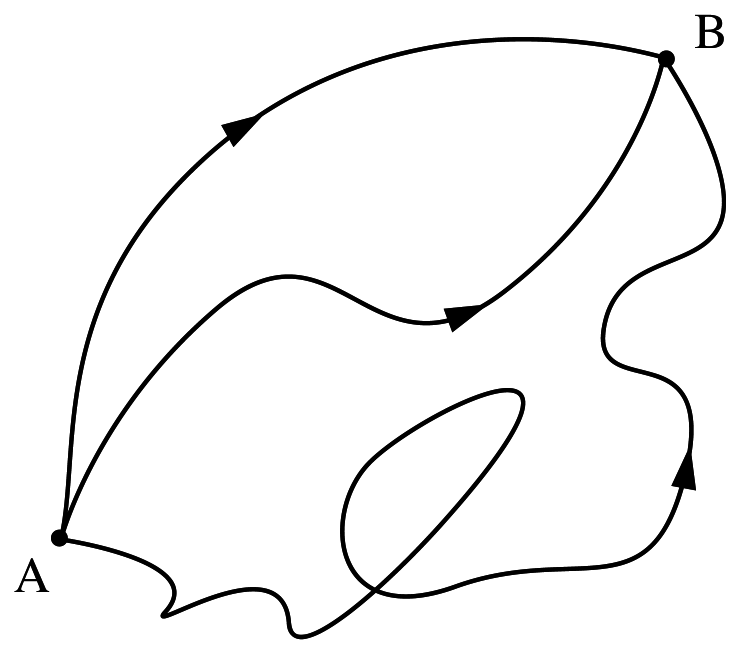
\includegraphics[scale=0.2]{DataForPresentation/PathIntegralSmooth.png}\footfullcite{Wikipdeia:PathIntegral}
    }
\end{frame}

\begin{frame}{Theory - Discrete Time Lattice}
    \only<2>
    {
        \centering
        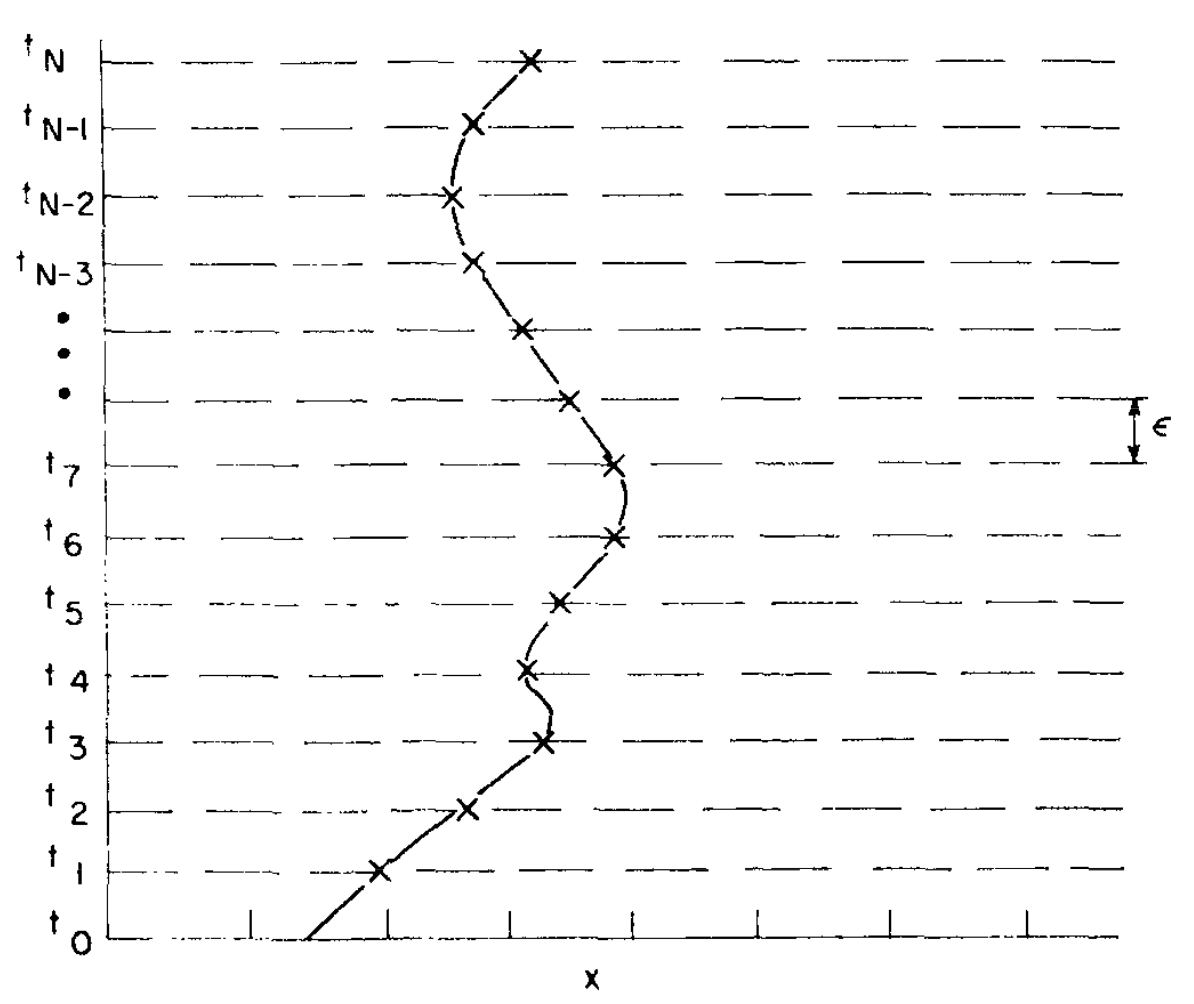
\includegraphics[scale=0.3]{dataForPresentation/PathIntegralDiscrete.png}\footfullcite{creutz_freedman_1981}
    }
    \only<3-4>
    {
        
        \begin{block}{Discrete Notation}
            \only<3-4>
            {
                \begin{align}
                & x\left(t_j\right) = x_j \\ 
                \only<4>
                {
                    & t_{j+1} -t_j = \epsilon
                }
                \end{align}
            }
        \end{block}
    }
    \only<5->
    {
        
        \begin{block}{Discrete Action}
            \begin{equation}
                S = \sum^{N-1}_{j=0} \epsilon \left[\frac{1}{2}m\frac{\left(x_{j+1}-x_j\right)^2}{\epsilon^2}-V\left(x_j\right)\right]
            \end{equation}
        \end{block}
    }
    \only<6->
    {
        
        \begin{block}{Discrete Path Integral}
            \begin{equation}
                \braket{x_b,t_b|x_a,t_a} \sim \int^{\infty}_{-\infty}\prod^{N-1}_{j=1}dx_{j} \exp{\left(\frac{i}{\hbar}S\left\{x_j\right\}\right)}
            \end{equation}
        \end{block}
    }
\end{frame}

\begin{frame}{Theory - Connecting to Statistical Mechanics}
    \only<2-4>
    {
        \begin{block}{Wick Rotation}
            \only<2-4>
            {
                \begin{equation}
                     \tau = it
                \end{equation}
            }
            \only<3-4>
            {
                \begin{equation}
                    a = i \epsilon
                \end{equation}
            }
        \end{block}
    }
    \only<4-5>
    {
        \begin{block}{Discrete Euclidean Action}
            \only<4-5>
            {
                \begin{equation}
                    S = i \sum^{N-1}_{j=0} a \left[\frac{1}{2}m\frac{\left(x_{j+1}-x_j\right)^2}{a}+V\left(x_j\right)\right] \coloneqq iS_E
                \end{equation}
            }
        \end{block}
    }
    \only<5->
    {
        \begin{block}{Discrete Euclidean Path Integral}
            \only<5->
            {
                \begin{equation}
                    \braket{x_b,t_b|x_a,t_a} \sim \int^{\infty}_{-\infty}\prod^{N-1}_{j=1}dx_{j} \exp{\left(-\frac{1}{\hbar}S_E\left\{x_j\right\}\right)}
                \end{equation}
            }
        \end{block}
    }
    \only<6->
    {
        \begin{block}{Partition Function}
            \only<6->
            {
                \begin{equation}
                    Z \sim \int^{+\infty}_{-\infty} \prod^{N-1}_{j=1} dx_i \exp{\left(-\beta H\left(\left \{x_i\right \}\right)\right)}
                \end{equation}
            }
        \end{block}
    }
\end{frame}

\section{Numerics}
\begin{frame}{Numerics - Monte Carlo}
    \only<2->
    {
        \begin{block}{Monte Carlo Estimate}
            \begin{equation}
                \bar{A} = \frac{1}{M}\sum^{M}_{\nu = 1} A\left(\bm{x}_{\nu}\right)
            \end{equation}
        \end{block}
    }
    \only<3->
    {
        \begin{block}{Boltzmann Distribution}
            \begin{equation}
                p\left(\bm{x}_{\nu}\right){\cal D}\bm{x} = \frac{\exp{\left(-S\left(\bm{x}_{\nu}\right)\right)}{\cal D}\bm{x}}{\int {\cal D}\bm{x}\exp{\left(-S\left(\bm{x}\right)\right)}}
            \end{equation}
        \end{block}
    }
\end{frame}


\begin{frame}{Numerics - Hybrid Monte Carlo Algorithm}
    \only<2-3>
    {
        \begin{block}{Fictitious Momenta}
            \begin{equation}
                p_i , i = 0 \dots {N-1}
            \end{equation}
        \end{block}
    }
    \only<3>
    {
        \begin{block}{HMC Hamiltonian}
            \begin{equation}
                H_{hmc} \coloneqq \sum_{i=0}^{N-1} \frac{ p_{i}^{2} } {2m} + S\left(\left\{x_i\right\}\right)
            \end{equation}
        \end{block}
    }

    \only<4->
    {
        \begin{block}{HMC Algorithm}
            \begin{enumerate} 
                \setcounter{enumi}{-1}

                \item<4-> Provide configuration $\left\{q_i\right\}$.

                \item<5-> Generate $\left\{p_i\right\}$ from $\mathcal{N}\left(0, 1\right)$.

                \item<6-> Evolve $\left(\left\{q_i \right\}, \left\{p_i \right\}\right)$ using Hamilton's equations to a final state $\left(\left\{q_i^*\right\}, \left\{p_{i}^{*} \right\}\right)$

                \item<7-> Accept configuration $ \left \{ q_{i}^{*} \right \} $ with probability $ \min{ \left [ 1 , \exp{ \left ( - H_{HMC} \left ( \left \{ q_{i}^{*} \right \} ,\left \{ p_{i}^{*} \right \} \right) + H_{HMC} \left ( \left \{ q_{i} \right \}, \left \{ p_{i} \right \} \right ) \right ) } \right ] } $ (Metropolis update).

                \item<8-> Return to step $1$.
            \end{enumerate}
        \end{block}
    }    
\end{frame}
    

\section{Results}

\begin{frame}{Results - Harmonic Oscillator Expectation Values}
    \only<2->{
        \begin{figure}
            \begin{table}
                \begin{tabular}{|c|c|c|c|}
                    \hline
                    Value & Measured & Discrete Theory\footfullcite{creutz_freedman_1981} & Continuum Theory \\ \hline\hline\noalign{\pause}
                    $\braket{x}$   & $0.00015(20) $ &  $0$            & $0$    \\ \hline\noalign{\pause} 
                    $\braket{x^2}$ & $0.44723(14) $ &  $0.4472135955$ & $0.5$  \\ \hline\noalign{\pause} 
                    $E_0$          & $0.44723(14) $ &  $0.4472135955$ & $0.5$  \\ \hline\noalign{\pause} 
                    $E_1$          & $0.9679(90)  $ &  $FILL$ & $1$  \\ \hline 
                \end{tabular}
                \note[item]{Expectation Values for quantum harmonic oscillator with $\mu^2 = 1$, $m=1$, $\text{lattice spacing} = 1$, $\text{lattice size} = 1000$,$\text{leapfrog step size} = 0.1$, $\text{leapfrog steps} = 10$, $\text{configurations}=100000$,$\text{burn period} = 1000 $}
            \end{table}
        \end{figure}
    }
\end{frame}

\begin{frame}{Results - Harmonic Oscillator Potential}
    \only<2->{\begin{figure}
    \centering
        \begin{tikzpicture}
            \begin{axis}[
                legend style={font=\tiny},
                xlabel= {$x$},
                ylabel style ={rotate=-90},
                ylabel= {$V(x)$},
                enlargelimits=true,
                ]
                \addplot[domain=-4:4, samples=100, color=black,]{0.5*x^2};
                \addlegendentry{$V(x)=\frac{\mu^2}{2}x^2$}

            \end{axis}
        \end{tikzpicture}
        \note[item]{Harmonic Oscillator Potential with $\mu^2 = 1$.}
    \end{figure}}
\end{frame}

\begin{frame}{Results - Harmonic Oscillator Wave Function}
    

    \only<4-6>{\begin{block}{Discrete Wave Function\footfullcite{creutz_freedman_1981}}
    \only<4-6>{
    
        \begin{equation}
            \psi_{disc.}{\left(x\right)} = \left(\frac{\omega}{\pi}\right)^\frac{1}{4}\exp{\left(-\frac{1}{2}\omega x^2\right)}
        \end{equation}
    }
    
    \only<5-6>{
    \begin{equation}
    \omega^2 = \mu^2\left(1+\frac{a^2 \mu^2}{4}\right)
    \end{equation}}
    \only<6>{
    \begin{equation}
    \left| \psi_{disc.}{\left(x\right)} \right|^2 = \sqrt{\frac{\sqrt{5}}{2\pi}}\exp{\left(-\frac{1}{2}\sqrt{5}{\omega} x^2\right)}
    \end{equation}}
    \end{block}}
    \only<9-10>{\begin{block}{Continuous Wave Function}
    \only<9-10>{
    \begin{equation}
    \psi_{cont.}{\left(x\right)} = \left(\frac{\mu}{\pi}\right)^\frac{1}{4}\exp{\left(-\frac{1}{2}\mu x^2\right)}
    \end{equation}}
    \only<10>{
    \begin{equation}
    \left| \psi_{cont.}{\left(x\right)} \right|^2 = \frac{1}{\sqrt{2\pi}}\exp{\left(-x^2\right)}
    \end{equation}}
    \end{block}}

    \only<2,7,11->{\begin{figure}
    \centering
        \begin{tikzpicture}
            \begin{axis}[
                legend style={font=\tiny},
                xlabel= {$x$},
                ylabel style ={rotate=-90},
                ylabel= {$\left|\psi{\left(x \right)}\right|^2$},
                enlargelimits=true,
                ]
                \only<2,7,11->{\addplot[only marks, 
                                   mark=x,color=black]
                            plot [error bars/.cd, 
                                    y dir = both, 
                                    y explicit]
                            table[x index=0, 
                                  y index=1, 
                                  y error index=2]{DataForPresentation/HarmonicWaveFunction.dat};
                    \addlegendentry{Measured Values}}
                \only<7,11->{\addplot[domain=-4:4,
                         samples=100,
                         color=blue,
                         ]
                         {sqrt(sqrt(5)/(2*pi))*e^(-0.5*sqrt(5)*x*x)};
                         \addlegendentry{Discrete Theory}}
                \only<11->{\addplot[domain=-4:4,
                         samples=100,
                         color=red,
                         ]
                         {1/sqrt(pi)*e^-x*x};
                         \addlegendentry{Continuum Theory}}
                         

            \end{axis}
        \end{tikzpicture}
        \note[item]{Continuum, discrete and measured wave functions for the harmonic oscillator with $\mu^2 = 1, m = 1, a = 1, L = 1000, d = 0.1, N = 10, \text{configurations} = 100000, \text{burn period} = 1000$.}
    \end{figure}}
\end{frame}

\begin{frame}{Results - Harmonic Oscillator Typical Trajectory}
    \only<2->{\begin{figure}
    \centering
        \begin{tikzpicture}
            \begin{axis}[
                xlabel= {Lattice Site},
                ylabel style ={rotate=-90},
                ylabel= {$x$},
                enlargelimits=true,
                ]
                \addplot[color=black,mark=x,]
                    table[x index=0, y index=1]{DataForPresentation/HarmonicTypicalTrajectory.dat};

            \end{axis}
        \end{tikzpicture}
        \note[item]{Typical configuration for the harmonic oscillator with $\mu^2 = 1, m = 1, a = 1, L = 1000, d = 0.1, N = 10, \text{configurations} = 100000, \text{burn period} = 1000$.}
    \end{figure}}
\end{frame}

\begin{frame}{Results - Harmonic Oscillator Lattice spacing vs. $\braket{x^2}$}

    \only<3-4>{
        \begin{block}{$\braket{x^2}$ on a lattice \footfullcite{creutz_freedman_1981}}
            \only<3-4>{
                \begin{equation}
                    \braket{x^2} = \frac{1}{2\left(1+\frac{1}{4}a^2\right)^{\frac{1}{2}}}\left(\frac{1+R^n}{1-R^n}\right)
                \end{equation}
            }
    
            \only<4>{
                \begin{equation}
                    R = 1 + \frac{a^2\mu^2}{2}-a\mu\left(1+\frac{a^2\mu^2}{4}\right)^{\frac{1}{2}}
                \end{equation}}
        \end{block}
    }

    \only<2,5->{\begin{figure}
    \centering
        \begin{tikzpicture}
            \begin{axis}[
                legend style={font=\tiny},
                xlabel= {$a$},
                ylabel style ={rotate=-90},
                ylabel= {$\braket{x^2}$},
                enlargelimits=true,
                ]
                \only<2,5->{\addplot[only marks, 
                                   mark=x,color=black]
                            plot [error bars/.cd, 
                                    y dir = both, 
                                    y explicit]
                            table[x index=0, 
                                  y index=1, 
                                  y error index=2]{DataForPresentation/LatticeSpacingvsExpectationXSquared.dat};
                    \addlegendentry{Measured Values}}
                \only<5->{\addplot[domain=0:1,
                         samples=100,
                         color=blue,
                         ]
                         {(1/2)*(1/sqrt(1+0.25*x*x)) * ((1+(1+0.5*x*x-x*sqrt(1+0.25*x*x))^(1000))/((1-(1+0.5*x*x-x*sqrt(1+0.25*x*x))^(1000))))};
                         \addlegendentry{Discrete Theory}}
                         

            \end{axis}
        \end{tikzpicture}
        \note[item]{Relationship between lattice spacing and expectation of position squared for the harmonic oscillator with $\mu^2 = 1, m = 1, a = 1, L = 1000, d = 0.1, N = 10, \text{configurations} = 100000, \text{burn period} = 1000$.}
    \end{figure}}   
\end{frame}

\begin{frame}{Results - Anharmonic Oscillator Potential}
    \only<2->{\begin{figure}
    \centering
        \begin{tikzpicture}
            \begin{axis}[
                legend style={font=\tiny},
                xlabel= {$x$},
                ylabel= {$V(x)$},
                ylabel style ={rotate=-90},
                enlargelimits=true,
                ]
                \addplot[domain=-4:4, samples=100, color=black,]{x^4-8*x^2+16};
                \addlegendentry{$V(x)=\lambda\left(x^2-f^2\right)^2$}

            \end{axis}
        \end{tikzpicture}
        \note[item]{Anharmonic Oscillator Potential with $\lambda = 1, f^2 = 4$.}
    \end{figure}}
\end{frame}

\begin{frame}{Results - Anharmonic Oscillator Expectation Values}
    \only<2->{
        \begin{figure}
            \begin{table}
                \begin{tabular}{|c | c | c | c }
                    \hline
                    Value & Measured & Reference Values \footfullcite{blankenbecler_degrand_sugar_1980} \\ \hline\hline\noalign{\pause}
                    $\braket{x}$   & FILL &  $0$ \\ \hline\noalign{\pause}
                    $\braket{x^2}$ & FILL &  $FILL$ \\ \hline\noalign{\pause}
                    $E_0$          & FILL &  $FILL$ \\ \hline\noalign{\pause}
                    $E_1$          & FILL &  $FILL$ \\ \hline        
                \end{tabular}
                \note[item]{Expectation Values for quantum anharmonic oscillator with $\mu^2 = 1$, $\text{lattice spacing} = 1$, $\text{lattice size} = 1000$}
            \end{table}
        \end{figure}
    }
\end{frame}

\begin{frame}{Results - Anharmonic Oscillator Wave Function}
    \only<2->{\begin{figure}
    \centering
        \begin{tikzpicture}
            \begin{axis}[
                xlabel= {$x$},
                ylabel style ={rotate=-90},
                ylabel= {$\left|\psi{\left(x \right)}\right|^2$},
                enlargelimits=true,
                ]
                \addplot[color=black,mark=x,]
                    plot [error bars/.cd, y dir = both, y explicit]
                    table[x index=0, y index=1, y error index=2]{DataForPresentation/AnharmonicWaveFunction.dat};

            \end{axis}
        \end{tikzpicture}
        \note[item]{Measured wave function for the harmonic oscillator with $\lambda = 1, f^2=4 m = 1, a = 1, L = 1000, d = 0.01, N = 100, \text{configurations} = 100000, \text{burn period} = 1000$.}
    \end{figure}}
\end{frame}

\begin{frame}{Results - Anharmonic Oscillator Typical Trajectory}
    \only<2->{\begin{figure}
    \centering
        \begin{tikzpicture}
            \begin{axis}[
                xlabel= {Lattice Site},
                ylabel style ={rotate=-90},
                ylabel= {$x$},
                enlargelimits=true,
                ]
                \addplot[color=black,mark=x,]
                    table[x index=0, y index=1]{DataForPresentation/AnharmonicTypicalTrajectory.dat};

            \end{axis}
        \end{tikzpicture}
        \note[item]{Typical configuration for the anharmonic oscillator with $\lambda = 1, f^2 = 4, m = 1, a = 1, L = 1000, d = 0.01, N = 100, \text{configurations} = 100000, \text{burn period} = 1000$.}
    \end{figure}}
\end{frame}

\begin{frame}{Results - Isolated Modes Wave Function}
    \only<2->{\begin{figure}
    \centering
        \begin{tikzpicture}
            \begin{axis}[
                xlabel= {$x$},
                ylabel style={rotate=-90},
                ylabel= {$\left|\psi{\left(x \right)}\right|^2$},
                enlargelimits=true,
                ]
                \addplot[color=black,mark=x,]
                    plot [error bars/.cd, y dir = both, y explicit]
                    table[x index=0, y index=1, y error index=2]{DataForPresentation/IsolatedModesWaveFunction.dat};

            \end{axis}
        \end{tikzpicture}
        \note[item]{Measured wave function for the harmonic oscillator with $\lambda = 1, f^2=4 m = 1, a = 1, L = 1000, d = 0.2, N = 5, \text{configurations} = 20000, \text{burn period} = 1000$.}
    \end{figure}}
\end{frame}

\section{Conclusion}
\begin{frame}{Conclusion}
\begin{itemize}
  \item<2-> Did it work? 
    \begin{itemize}
        \item<3-> Successfully reproduced known values using HMC method.
    \end{itemize}
  \item<4-> What next?
    \begin{itemize}
        \item<5-> Introduce ``tempering'' into the dynamics to sample from isolated modes.
    \end{itemize}
  \item<6-> Applications of tempering?
  \begin{itemize}
        \item<7-> Potentially applicable to lattice field theory where computation time is far more costly.
    \end{itemize}
\end{itemize}
\end{frame}
\end{document}
